%%
%% Copyright 2007, 2008, 2009 Elsevier Ltd
%%
%% This file is part of the 'Elsarticle Bundle'.
%% ---------------------------------------------
%%
%% It may be distributed under the conditions of the LaTeX Project Public
%% License, either version 1.2 of this license or (at your option) any
%% later version.  The latest version of this license is in
%%    http://www.latex-project.org/lppl.txt
%% and version 1.2 or later is part of all distributions of LaTeX
%% version 1999/12/01 or later.
%%
%% The list of all files belonging to the 'Elsarticle Bundle' is
%% given in the file `manifest.txt'.
%%

%% Template article for Elsevier's document class `elsarticle'
%% with harvard style bibliographic references
%% SP 2008/03/01
%%
%%
%%
%% $Id: elsarticle-template-harv.tex 4 2009-10-24 08:22:58Z rishi $
%%
%%
%%\documentclass[preprint,authoryear,12pt]{elsarticle}

%% Use the option review to obtain double line spacing
\documentclass[authoryear,preprint,review,12pt]{elsarticle}

%% Use the options 1p,twocolumn; 3p; 3p,twocolumn; 5p; or 5p,twocolumn
%% for a journal layout:
%% \documentclass[final,authoryear,1p,times]{elsarticle}
%% \documentclass[final,authoryear,1p,times,twocolumn]{elsarticle}
%% \documentclass[final,authoryear,3p,times]{elsarticle}
%% \documentclass[final,authoryear,3p,times,twocolumn]{elsarticle}
%% \documentclass[final,authoryear,5p,times]{elsarticle}
%% \documentclass[final,authoryear,5p,times,twocolumn]{elsarticle}

%% if you use PostScript figures in your article
%% use the graphics package for simple commands
\usepackage{graphics}
\usepackage{longtable}
%% or use the graphicx package for more complicated commands
%% \usepackage{graphicx}
%% or use the epsfig package if you prefer to use the old commands
%% \usepackage{epsfig}

%% The amssymb package provides various useful mathematical symbols
\usepackage{amssymb}
%% The amsthm package provides extended theorem environments
\usepackage{amsthm}
\usepackage{colortbl}

% For psudo code
\usepackage{amsmath}
\usepackage{algorithm}
\usepackage[noend]{algpseudocode}
\usepackage{setspace}

\makeatletter
\def\BState{\State\hskip-\ALG@thistlm}
\makeatother

%% The lineno packages adds line numbers. Start line numbering with
%% \begin{linenumbers}, end it with \end{linenumbers}. Or switch it on
%% for the whole article with \linenumbers after \end{frontmatter}.
%% \usepackage{lineno}

%% natbib.sty is loaded by default. However, natbib options can be
%% provided with \biboptions{...} command. Following options are
%% valid:

%%   round  -  round parentheses are used (default)
%%   square -  square brackets are used   [option]
%%   curly  -  curly braces are used      {option}
%%   angle  -  angle brackets are used    <option>
%%   semicolon  -  multiple citations separated by semi-colon (default)
%%   colon  - same as semicolon, an earlier confusion
%%   comma  -  separated by comma
%%   authoryear - selects author-year citations (default)
%%   numbers-  selects numerical citations
%%   super  -  numerical citations as superscripts
%%   sort   -  sorts multiple citations according to order in ref. list
%%   sort&compress   -  like sort, but also compresses numerical citations
%%   compress - compresses without sorting
%%   longnamesfirst  -  makes first citation full author list
%%
%% \biboptions{longnamesfirst,comma}

% \biboptions{}

\journal{Expert Systems with Applications}

\newtheorem{definition}{Definition}
\newtheorem{proposition}{Proposition}

\begin{document}

\begin{frontmatter}

%% Title, authors and addresses

%% use the tnoteref command within \title for footnotes;
%% use the tnotetext command for the associated footnote;
%% use the fnref command within \author or \address for footnotes;
%% use the fntext command for the associated footnote;
%% use the corref command within \author for corresponding author footnotes;
%% use the cortext command for the associated footnote;
%% use the ead command for the email address,
%% and the form \ead[url] for the home page:
%%
%% \title{Title\tnoteref{label1}}
%% \tnotetext[label1]{}
%% \author{Name\corref{cor1}\fnref{label2}}
%% \ead{email address}
%% \ead[url]{home page}
%% \fntext[label2]{}
%% \cortext[cor1]{}
%% \address{Address\fnref{label3}}
%% \fntext[label3]{}

\title{A New Fast Hardware Software Platform for Computing Irreducible Testors}

%% use optional labels to link authors explicitly to addresses:
%% \author[label1,label2]{<author name>}
%% \address[label1]{<address>}
%% \address[label2]{<address>}


\address{Computer Science Department}
\address{National Institute for Astrophysics, Optics and Electronics}
\address{Sta. Ma. Tonanzintla, Puebla, 72840, Mexico}

\begin{abstract}
Feature selection is an important task in pattern recognition and decision-making systems. Given a dataset
described by a set of features, minimal subsets of features that preserve the ability to discern between
objects from different classes are needed. The computation of these minimal subsets is a problem whose space 
complexity grows exponentially regarding the number of attributes. 
Several hardware architectures has been developed in order to reduce the execution time of existing algorithms,
making accessible larger datasets than those that software applications can solve.
%Testor Theory is a convenient way to solve this problem. A testor is defined as a subset of attributes that can discern between objects of different classes; and an irreducible testor is a minimal subset with this property. 
%Although there are efficient algorithms for computing irreducible testors, hardware implementations of these algorithms can improve their performance; taking advantage of the inherent parallelism in the evaluation of testor candidates. 
In this paper, a new fast hardware software platform for computing minimal subsets of features is presented.
This new approach, uses a pruning strategy that reduces the search space more than any other existing alternative,
in most cases.
Results from a prototype implementation, showing the runtime reduction achieved by the proposed platform, are
presented and discussed.

\end{abstract}

\begin{keyword}
%% keywords here, in the form: keyword \sep keyword
Feature Selection \sep Testor Theory \sep Hardware Architecture \sep
FPGA
%% MSC codes here, in the form: \MSC code \sep code
%% or \MSC[2008] code \sep code (2000 is the default)

\end{keyword}

\end{frontmatter}

% \linenumbers

%% main text
\section{Introduction}
\label{sect:1}

Feature selection for supervised classification consists in identifying those attributes that 
provide relevant information for the classification process. This procedure does not only reduce the 
computational cost of the classification process by eliminating superfluous information, but in some cases 
it could even provide better classification accuracy. 
Testor Theory can be used for feature selection as shown in~\citep{R27,R5}. A testor is defined as a subset of attributes that can discern objects from different classes. An irreducible testor is a subset of features such that every attribute is indispensable for satisfying the testor condition. Finding all irreducible testors has been proven as an NP-hard problem~\citep{R40}.

Feature selection is also a key aspect in expert and intelligent systems. \cite{Mart07} used Testor Theory to
propose a new case-based approach to help elaborate intelligents teaching-learning systems.  Irreducible testors
are computed in~\citep{Med07} to select problem variables in the proposal of an intelligent tutoring system with
the capacity to adapt the interaction to its user's specific needs. Recently, \cite{Torr14} used testors to 
determining factors associated with transfusion related acute lung injury. Another approach to feature selection,
the Rough Sets Reducts, has been found to have a close relation with irreducible testors~\citep{Lazo15}. Expert
systems can benefit also from Rough Sets methods, specially the feature selection by means of reducts, as shown 
by \cite{Yah00}.

Recently, there is an increasing popularity of architectures based on Field Programmable Gate-Array (FPGA) 
for solving complex computational problems. Several hardware software platforms based on this technology have 
been reported \citep{R29,R30}. 
In these platforms, the software component handles those tasks less suited for hardware implementation, 
and it is also responsible of configuring the FPGA, as well as handling communication with the hardware component. 
The hardware component, on the other hand, performs those operations with a high parallelism degree.

In spite of advances in the theoretical aspects of computing
irreducible testors \citep{R5,R8,R9}, there are 
no hardware implementations reported aside from \citep{R10,R11,R21}.
In the first work, an FPGA-based brute force approach for computing testors was proposed
\citep{R10}. This first approach did not take advantage of dataset characteristics to reduce the number 
of candidates to be tested; thus all $2^n$ combinations of $n$ features have to be tested. 
Then, in \citep{R11} a hardware architecture of the BT algorithm for computing irreducible testors was implemented. 
This algorithm uses a candidate pruning process for avoiding many unnecessary candidate evaluation, 
reducing the number of verifications of the irreducible testor condition. 
These two previous works computed a set of testors on the FPGA device whilst irreducible condition 
was evaluated afterwards by the software component in the hosting PC. 
Thus \cite{R21} proposed a hardware software platform for computing irreducible testors that 
implemented the BT algorithm, as in \citep{R11}, but it also included a new module that eliminates most of 
the non irreducible testors before transferring them to a host software application for final filtering. 
One disadvantage of these approaches is the huge amount of data that must be transferred to the PC.  
Consequently, in~\citep{Rod14} we proposed a modification to this platform in order to compute irreducible 
testors in the hardware component. 

Several hardware accelerations has been recently reported for feature selection in Rough Sets Theory. Authors of
\citep{Grze13,Kop14} presented an FPGA based platform for computing a reduct. \cite{Tiwari13} presented various
algorithms for attribute reduction using concepts of Rough Sets Theory and implemented the Quick Reduct
algorithm in a hardware fashion. Then, \cite{Tiwari14} presented a thorough survey on hardware implementation 
of rough set algorithms. Unfortunately, these hardware implementations aim to compute a single reduct. 
\cite{Jensen14} addressed the lack of guarantees of finding a features subset with minimal cardinality, as the
main drawback of these approaches. Furthermore, the problem of computing a single reduct has not exponential
complexity. Hardware accelerations of these algorithms are intended to be applied on realtime applications
where feature selection must be dynamically accomplished.

In this paper, we present an efficient hardware software platform for computing irreducible
testors using the CT-EXT algorithm proposed in~\citep{R22}. The contribution of this
work is the design and implementation of a hardware architecture that traverses the search space in a 
different order than that presented in \citep{R11, R21,Rod14}. This new strategy evaluates less candidate
subsets than previous architectures, which results in shorter runtime. In comparison to the 
software versions of CT-EXT~\citep{R22, R23}, our proposal evaluates a candidate every clock cycle for
a fastest execution. The runtime gain of our new hardware software platform is demonstrated throughout
experiments over synthetic datasets. 
%CT-EXT has proven being, in most cases, more efficient in finding irreducible testors than BT~\citep{R22, R23}.

%The intensive computational requirements due to the exponential
%complexity, regarding the number of attributes, of the CT-EXT algorithm,
%can be met by a combination of technological improvements and efficient hardware architectures based on 
%parallel computational models. 

The rest of this paper is structured as follows. Section~\ref{sect:2} introduces the basic concepts of 
Testor Theory and the CT-EXT algorithm. Section~\ref{sect:3} introduces the proposed architecture.  
Evaluation of the proposed platform and a discussion of the experimental results are 
presented in section~\ref{sect:6}. Finally, section~\ref{sect:8} shows our conclusions and some directions 
for future work.

\section{Basic concepts}
\label{sect:2}

In pattern recognition, feature selection is a very important task for supervised classification. In the logical
 combinatorial approach to pattern recognition \citep{R5}, a useful
way to deal with this problem is through Testor Theory. The concept of testor for pattern recognition was
introduced by \cite{R12}. They defined a testor as a subset of features that allows
differentiating objects from different classes. Testors are quite useful, especially when object descriptions
contain both numeric and non-numeric features, and maybe they are incomplete (mixed incomplete data)
\citep{R5}. This concept has been developed in different contexts \citep{R1}. From an 
algorithmic point of view, Testor Theory has shown a continuous development from its origins to the present 
\citep{R31,R13,R23}.

Let $TM$ be a training matrix with $k$ objects described through $n$
features of any type $\{x_{1},\ldots,x_{n}\}$ and grouped in $r$
classes. Let $DM$ be a Boolean dissimilarity matrix (0 = similar, 1 =
dissimilar), obtained from feature by feature comparisons of every
pair of objects from $TM$ belonging to different classes. $DM$ has
$m$ rows and $n$ columns, where usually $m>>k$.

Let $T$ be a subset of attributes. Testors and irreducible testors are formally defined as follows:

\begin{definition} \label{def1}
$T$ is a testor if and only if when all
features (columns) are eliminated from $DM$, except those from $T$, there is
not any row of $DM$ with only 0's. $T$ is an irreducible testor if none of its proper subsets is a testor.
\end{definition}

In defintion \ref{def1}, if there is not any row of $DM$ with only
0's it means that there is not a pair of objects from different
classes that are similar on all the features of $T$, that is, a
testor $T$ allows differentiating objects from different
classes. From definition~\ref{def1}, if $T$ is a testor then, any superset of $T$ is a testor too.

The number of rows in $DM$ could be too large, therefore a strategy to reduce this matrix, without losing
relevant information for computing irreducible testors, is eliminating redundant rows \citep{R1}.

%% DEFINICION 
\begin{definition}
Let $f=[f_1, f_2, \dots , f_n]$ and $f'=[f'_1, {f'}_2, \dots , {f'}_n]$ be two rows of $DM$, $f$ 
is a sub-row of $f^{'}$ if for each column $j=1,2,\dots ,n$;  $f_{j} \le f'_{j}$ and for at least one index, the 
inequality is strict.
\end{definition}

%% DEFINICION 
\begin{definition}
A row $f$ of $DM$ is a basic row if no row of the matrix $DM$ is a sub-row of $f$. 
\end{definition}

%% DEFINICION 
\begin{definition}
The basic matrix of $DM$, denoted as $BM$, is the sub-matrix of $DM$ formed only by the basic rows (without 
repetitions).

\end{definition}

Let $TT(DM)$ and $TT(BM)$ be the sets of all irreducible testors of $DM$ and $BM$ respectively, it is 
relatively easy to prove that $TT(DM)=TT(BM)$, see \citep{R32}; i.e., we can conclude that usually $DM$ 
contains redundant information. In addition, the construction of $BM$ from $DM$ is a very fast process, 
then we work over $BM$.

The CT-EXT algorithm has the following theoretical bases.
\begin{definition} \label{def21} Let $f_i$ be a row of BM, $f_i$ is a zero row of $S \subseteq R$, and we denote it as ${f_i}^0 (S)$, if $\forall x_p \in S$, $f_i [p] = BM [i, p] = 0$. We denote as $\Sigma_S f^0$  the amount of zero rows of S.
\end{definition}
\begin{definition} \label{def22} In terms of BM, a testor $T \subseteq R$ is a feature set such that there
are no zero rows of T in BM. 
\end{definition}
\begin{definition} \label{def23} Let $f_i$ be a row of BM, $f_i$ is a typical row of $S \subseteq R$ regarding $x_q$, being $x_q \in S$, and we denote it by ${f_i}^1 (S,q)$ if $f_i [q] = BM [i, q] = 1$, and $\forall x_p \in S$, $x_p \neq x_q$ , $f_i [p] = BM [i, p] =~0$.
\end{definition}

\begin{definition} \label{def24} In terms of BM, $T \subseteq R$ is an irreducible testor if T is a testor and
$\forall x_j \in T, \exists {f_i}^1 (T, j)$.
\end{definition}

This means that for each feature in an irreducible testor, there exists a row in 
the sub matrix of $BM$ associated to $T$, having a 1 in the position corresponding
to that feature, and 0 in all remaining positions (if any column of $T$ is eliminated, 
at least one zero row will appear, and the testor property would not be fulfilled). 

\begin{definition} \label{def25} Given $T \subseteq R$ and $x_j \in R$ such that $x_j \notin T$. 
%We denote as $\sum_T f^0$ the amount of zero rows of T. 
We say that $x_j$ contributes to T if, and only if, $\sum_{T\cup\{x_j\}} f^0 < \sum_T f^0$.
\end{definition}
This definition indicates that a feature contributes to a feature subset $T$
if for at least one zero row in $BM$, considering only $T$, the new feature has a 1 in 
this row. So, adding this feature to $T$, there are less
zero rows than the amount of zero rows for $T$.

It is easy to see that $\sum_T f^0 \geq \sum_{T\cup\{x_j\}} f^0$. If we
increase the feature subset, either the zero rows are maintained, and in this
case the column added does not contribute to the combination, or the number of zero rows decreases.

Propositions~\ref{prop1} and~\ref{prop2} are important conclusions for CT-EXT which were introduced and 
proved in \citep{R22}.

\begin{proposition}\label{prop1} Given $T \subseteq R$ and  $x_j \in R$ such that $x_j \notin T$. If $x_j$ does not contribute to T, then $T\cup\{x_j\}$ cannot be a subset of any irreducible testor.
\end{proposition}

\begin{proposition}\label{prop2} Given $T \subseteq R$ and $Z \subseteq R$ such that $Z \cup T \neq T$. If T is a testor, 
then $T \cup Z$ is a testor too, but it is not an irreducible testor.
\end{proposition}

\subsection{CT-EXT algorithm}
Algorithm~\ref{ctext_algo} exposes the pseudo code for CT-EXT, a detailed explanation for 
this algorithm can be seen in~\citep{R22}. The function SortBM$(BM)$ sorts the basic matrix as follows.
Randomly select one of the rows of $BM$ with the fewest number of 1's. The selected row goes first and 
all columns in which it has a 1 are moved to the left.  

The function Evaluate$(BM,T)$ returns three values: $testor$, $irreducible$ and $zero\_rows$. $testor$ is TRUE if the set $T$ is a testor of $BM$ and FALSE otherwise. $irreducible$ is TRUE if the set $T$ is an irreducible testor and FALSE otherwise. $zero\_rows$ is the amount of zero rows of $T$. The function LastOne($T$) returns the 
position of the rightmost element in the set $T$.

\begin{algorithm}
	\begin{spacing}{1.0}
	\begin{small}	
	\caption{CT-EXT algorithm}\label{ctext_algo}
	\begin{algorithmic}[1]	
		%\Procedure{CT-EXT}{}
		\State \textbf{Input: } $BM$ - basic matrix with $m$ rows and $n$ columns.
		\State \textbf{Output: } $TT$ - set of irreducible testors.
			
			\State $TT \gets \{\}$
			\State $j \gets 0$ \Comment{first feature from $BM$ to be analyzed}
			\State $BM \gets$ SortBM$(BM)$
			
			\While{$BM[0,j] \neq 0$}\label{row1condition}
				\State $T \gets \{X_j\}$ \Comment{current feature subset}
				\State $testor, irreducible, zero\_rows \gets$ Evaluate$(BM,T)$
				\If{$testor=TRUE$}
					\If{$irreducible=TRUE$} \Comment{$T$ is an irreducible testor}
						\State $TT \gets TT \cup T$
					\EndIf
				\Else
					\State $i \gets j+1$
					\While{$i < n$}
						\State $T \gets T \cup \{X_i\}$
						\State $zero\_rows\_last \gets zero\_rows$
						\State $testor, irreducible, zero\_rows \gets$ Evaluate$(BM,T)$
						\If{$zero\_rows = zero\_rows\_last$} 
							\State $T \gets T \setminus \{X_i\}$ \Comment{attribute $X_i$ does not contributes}
						\Else
							\If{$testor=TRUE$}
								\If{$irreducible=TRUE$}
									\State $TT \gets TT \cup T$
								\EndIf
								\State $T \gets T \setminus \{X_i\}$
								\State $zero\_rows \gets zero\_rows\_last$
							\EndIf
						\EndIf
						\If{$i = n-1$}
							\State $k \gets$ LastOne($T$)
							\If{$k = i$}
								\State $T \gets T \setminus \{X_k\}$
								\State $k \gets$ LastOne($T$)
							\EndIf
							\If{$k \neq j$}
								\State $T \gets T \setminus \{X_k\}$
								\State $testor, irreducible, zero\_rows \gets$ Evaluate$(BM,T)$
								\State $i \gets k+1$
							\Else
								\State $i \gets i+1$
							\EndIf
						\Else
							\State $i \gets i+1$
						\EndIf
					\EndWhile
				\EndIf
				\State $j \gets j+1$
			\EndWhile
		%\EndProcedure
	\end{algorithmic}
	\end{small}
	\end{spacing}
\end{algorithm}

Example. Let us consider the basic matrix of Table~\ref{table1}, with $m=3$ rows and $n=5$ attributes. After the  ordering step we obtain the matrix shown in Table~\ref{table2}. Table~\ref{tab_example} illustrates the 
application of the CT-EXT algorithm over this basic matrix.

\begin{table}[!htb]
    \begin{minipage}{.5\linewidth}
      \caption{Basic Matrix for the example.}\label{table1}
      \centering
        \begin{tabular}{ ccccc }
 			\hline                       
  			$x_0$ & $x_1$ & $x_2$ & $x_3$ & $x_4$ \\
  			\hline
  			1 & 0 & 0 & 1 & 1 \\
  			0 & 1 & 1 & 0 & 1 \\
  			1 & 1 & 0 & 0 & 1 \\
  			\hline  
		\end{tabular}
    \end{minipage}%
    \begin{minipage}{.5\linewidth}
      \centering
        \caption{Ordered Basic Matrix obtained from the matrix of Table~\ref{table1}.}\label{table2}
        \begin{tabular}{ ccccc }
 			\hline                       
  			$x_0$ & $x_3$ & $x_4$ & $x_1$ & $x_2$ \\
  			\hline
  			1 & 1 & 1 & 0 & 0 \\
  			0 & 0 & 1 & 1 & 1 \\
  			1 & 0 & 1 & 1 & 0 \\
  			\hline  
		\end{tabular}
    \end{minipage} 
\end{table}

\newcommand{\lcell}[2][2in]{$\vcenter{\hsize#1\baselineskip11pt\vspace*{2.5pt}\raggedright#2\strut}$}

      %\centering
        \begin{longtable}{cccccl}
		\caption[CT-EXT example.]{CT-EXT algorithm example.} \label{tab_example} \\
 			\hline                       
  			\multicolumn{1}{>{\centering\arraybackslash}m{.12in}}{$T$} & 
  			\multicolumn{1}{>{\centering\arraybackslash}m{.5in}}{\scriptsize{Evaluate $(BM,T)$}} &
  			\multicolumn{1}{>{\centering\arraybackslash}m{.15in}}{$x_j$} & 
  			\multicolumn{1}{>{\centering\arraybackslash}m{.6in}}{\scriptsize{$T\cup\{x_j\}$}} &
  			\multicolumn{1}{>{\centering\arraybackslash}m{.8in}}{\scriptsize{Evaluate $(BM,T\cup\{x_j\})$}} & 
  			\multicolumn{1}{>{\centering\arraybackslash}m{1in}}{Comments}\\
  			\hline
  			$\{~\}$ & F, F, $\infty$ & $x_0$ & $\{x_0\}$ & F, F, 1 & 
  			\scriptsize{\lcell{$\{x_0\}$ is not a testor. Add a new attribute.}}\\
  			$\{x_0\}$ & F, F, 1 & $x_3$ & $\{x_0,x_3\}$ & F, F, 1 &
  			\scriptsize{\lcell{$x_3$ does not contribute. Eliminate $x_3$. Add a new attribute.}}\\
  			$\{x_0\}$ & F, F, 1 & $x_4$ & $\{x_0,x_4\}$ & T, F, 0 &
  			\scriptsize{\lcell{$x_4$ contributes, $\{x_0,x_4\}$ is testor but is not irreducible.
  			 	Eliminate $x_4$. Add a new attribute.}}\\
  			$\{x_0\}$ & F, F, 1 & $x_1$ & $\{x_0,x_1\}$ & T, T, 0 &
  			\scriptsize{\lcell{$x_1$ contributes, $\{x_0,x_1\}$ is an irreducible testor.
  				It is saved ($TT = \{\{x_0,x_1\}\}$).
  			 	Eliminate $x_1$. Add a new attribute.}}\\
  			$\{x_0\}$ & F, F, 1 & $x_2$ & $\{x_0,x_2\}$ & T, T, 0 &
  			\scriptsize{\lcell{$x_2$ contributes, $\{x_0,x_2\}$ is an irreducible testor.
  				It is saved ($TT = \{\{x_0,x_1\},\{x_0,x_2\}\}$).
  			 	Eliminate $x_2$. Add a new attribute.}}\\
  			$\{x_0\}$ & \multicolumn{5}{>{\centering\arraybackslash}m{5in}}{All attributes tested. 
  			Eliminate $x_0$ and add a new one.}\\
  			\hline 
  			$\{~\}$ & F, F, $\infty$ & $x_3$ & $\{x_3\}$ & F, F, 2 & 
  			\scriptsize{\lcell{$\{x_3\}$ is not a testor. Add a new attribute.}}\\
  			$\{x_3\}$ & F, F, 2 & $x_4$ & $\{x_3,x_4\}$ & T, F, 0 &
  			\scriptsize{\lcell{$x_4$ contributes, $\{x_3,x_4\}$ is testor but is not irreducible.
  			 	Eliminate $x_4$. Add a new attribute.}}\\
  			$\{x_3\}$ & F, F, 2 & $x_1$ & $\{x_3,x_1\}$ & T, T, 0 &
  			\scriptsize{\lcell{$x_1$ contributes, $\{x_3,x_1\}$ is an irreducible testor.
  				It is saved ($TT = \{\{x_0,x_1\},\{x_0,x_2\},\{x_3,x_1\}\}$).
  			 	Eliminate $x_1$. Add a new attribute.}}\\
  			$\{x_3\}$ & F, F, 2 & $x_2$ & $\{x_3,x_2\}$ & F, F, 1 & 
  			\scriptsize{\lcell{$x_2$ contributes but $\{x_3,x_2\}$ is not a testor. Add a new attribute.}}\\
  			$\{x_3\}$ & \multicolumn{5}{>{\centering\arraybackslash}m{5in}}{All attributes tested. 
  			Eliminate $x_3$ and add a new one.}\\
  			\hline 
  			$\{~\}$ & F, F, $\infty$ & $x_4$ & $\{x_4\}$ & T, T, 0 & 
  			\scriptsize{\lcell{$\{x_4\}$ is an irreducible testor.
  				It is saved ($TT = \{\{x_0,x_1\},\{x_0,x_2\},\{x_3,x_1\},\{x_4\}\}$).
  			 	Eliminate $x_4$. Add a new attribute.}}\\
  			\hline  
  			$\{~\}$ & F, F, $\infty$ &  $\{x_1\}$ & \multicolumn{3}{>{\centering\arraybackslash}m{4in}}{
  			$x_1$ has a 0 in first row of $BM$, Algorithm finishes.}\\
  			\hline  
		\end{longtable}

\section{Proposed platform}
\label{sect:3}

Since algorithms for computing all irreducible testors have
exponential complexity regarding the number of attributes, 
software based implementations may take an unacceptable amount of time. 
A common stage to all algorithms for computing irreducible testors is 
the verification of each candidate combination over the basic matrix. 
This is an intrinsic parallel operation that a hardware implementation 
could take advantage of.
The time complexity of evaluating a candidate for the testor conditions is
$O(nm)$ and for the irreducible condition is $O(n^2m)$; where $n$ is the number of 
attributes and $m$ is the number of rows in the basic matrix. In the hardware
component, these conditions are simultaneously evaluated in a single clock cycle.
The novelty in this work relays on the Candidate Generator module. This new module
implements the lexicographic total order~\citep{R22} as in the CT-EXT algorithm.
This traversing order allows our proposal to evaluate less candidates than 
those evaluated by the existing hardware architectures; reducing, this way, the 
execution time.
%Our platform consists in the implementation of a
%hardware architecture for computing all irreducible testors based on
%the CT-EXT algorithm. 

The proposed platform is shown in Fig.\,\ref{figArq}. The platform comprises a host PC and 
an Atlys board populated with a FPGA Spartan-6 device \citep{R15}; which are connected through a USB cable. A custom developed software application,
running in the PC, handles all the processes needed to create the bitstream file to configure the FPGA device. The custom architecture implemented in the 
FPGA carries out all the calculations needed to generate the testors and sends the results to the PC where the users can then analize the results. A detailed description of all the platform components are given below.

\begin{figure}[htb]
    \begin{center}
       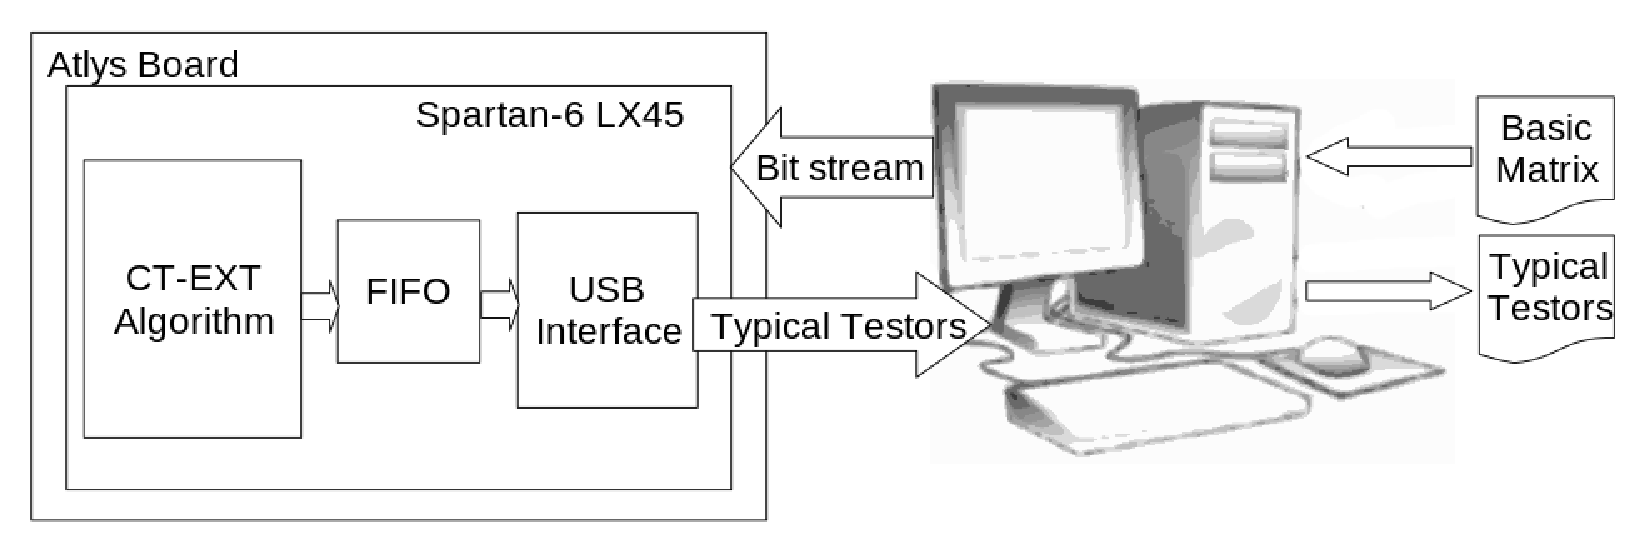
\includegraphics[width=13cm]{Arquitecture.eps}
    \end{center}
\caption{Proposed hardware software platform.}
\label{figArq}
\end{figure}

\subsection{Hardware architecture}
\label{sect:4}

\begin{figure}[htb]
    \begin{center}
        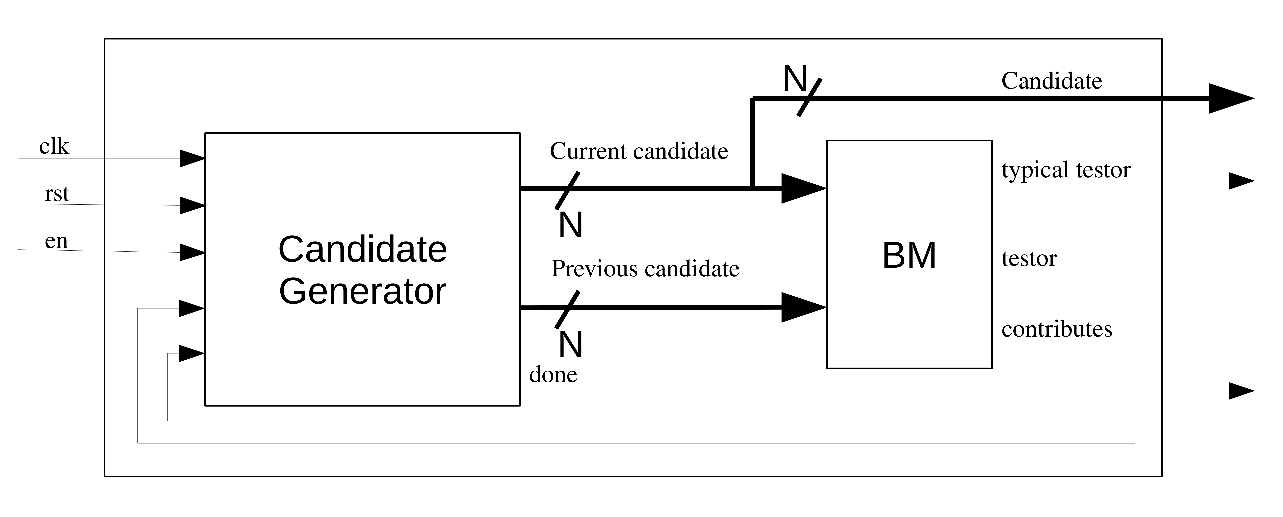
\includegraphics[width=13cm]{CT-ext_arq.eps}
    \end{center}
\caption{CT-EXT Architecture.}
\label{fig:3}
\end{figure}

In the hardware architecture, a feature subset is handled as an $n$-tuple, using a positional 
representation for all the $n$ attributes of a basic matrix $BM$. Given a subset $T$, its $n$-tuple representation 
has a 1 in the corresponding position $j$ for each $x_j \in T$ and 0 otherwise.
The process of deciding whether an $n$-tuple is a testor of $BM$ involves
comparing the candidate against each one of the $BM$'s rows. For
software-only implementations, this is a big disadvantage, specially for large 
matrices with many rows. The proposed hardware architecture exploits the parallelism 
inherent in the CT-EXT algorithm
and evaluates whether a candidate is an irreducible testor, or not, in a single
clock cycle. The hardware implementation of CT-EXT is composed of two modules, the BM module and the Candidate Generator module, as shown in
Fig.\,\ref{fig:3}. 

The $BM$ module stores the input matrix and
includes all the logic needed to decide whether an $n$-tuple is a testor. The candidate
generator module produces the candidates ($n$-tuples) to be
evaluated by the $BM$ module. In order to calculate the next candidate
according to the CT-EXT algorithm, the architecture feedbacks the
evaluation result of the previous candidate to the generator module;
this drastically reduces the number of candidates tested and
consequently the number of iterations needed by the algorithm. 


\begin{figure}[htb]
    \begin{center}
        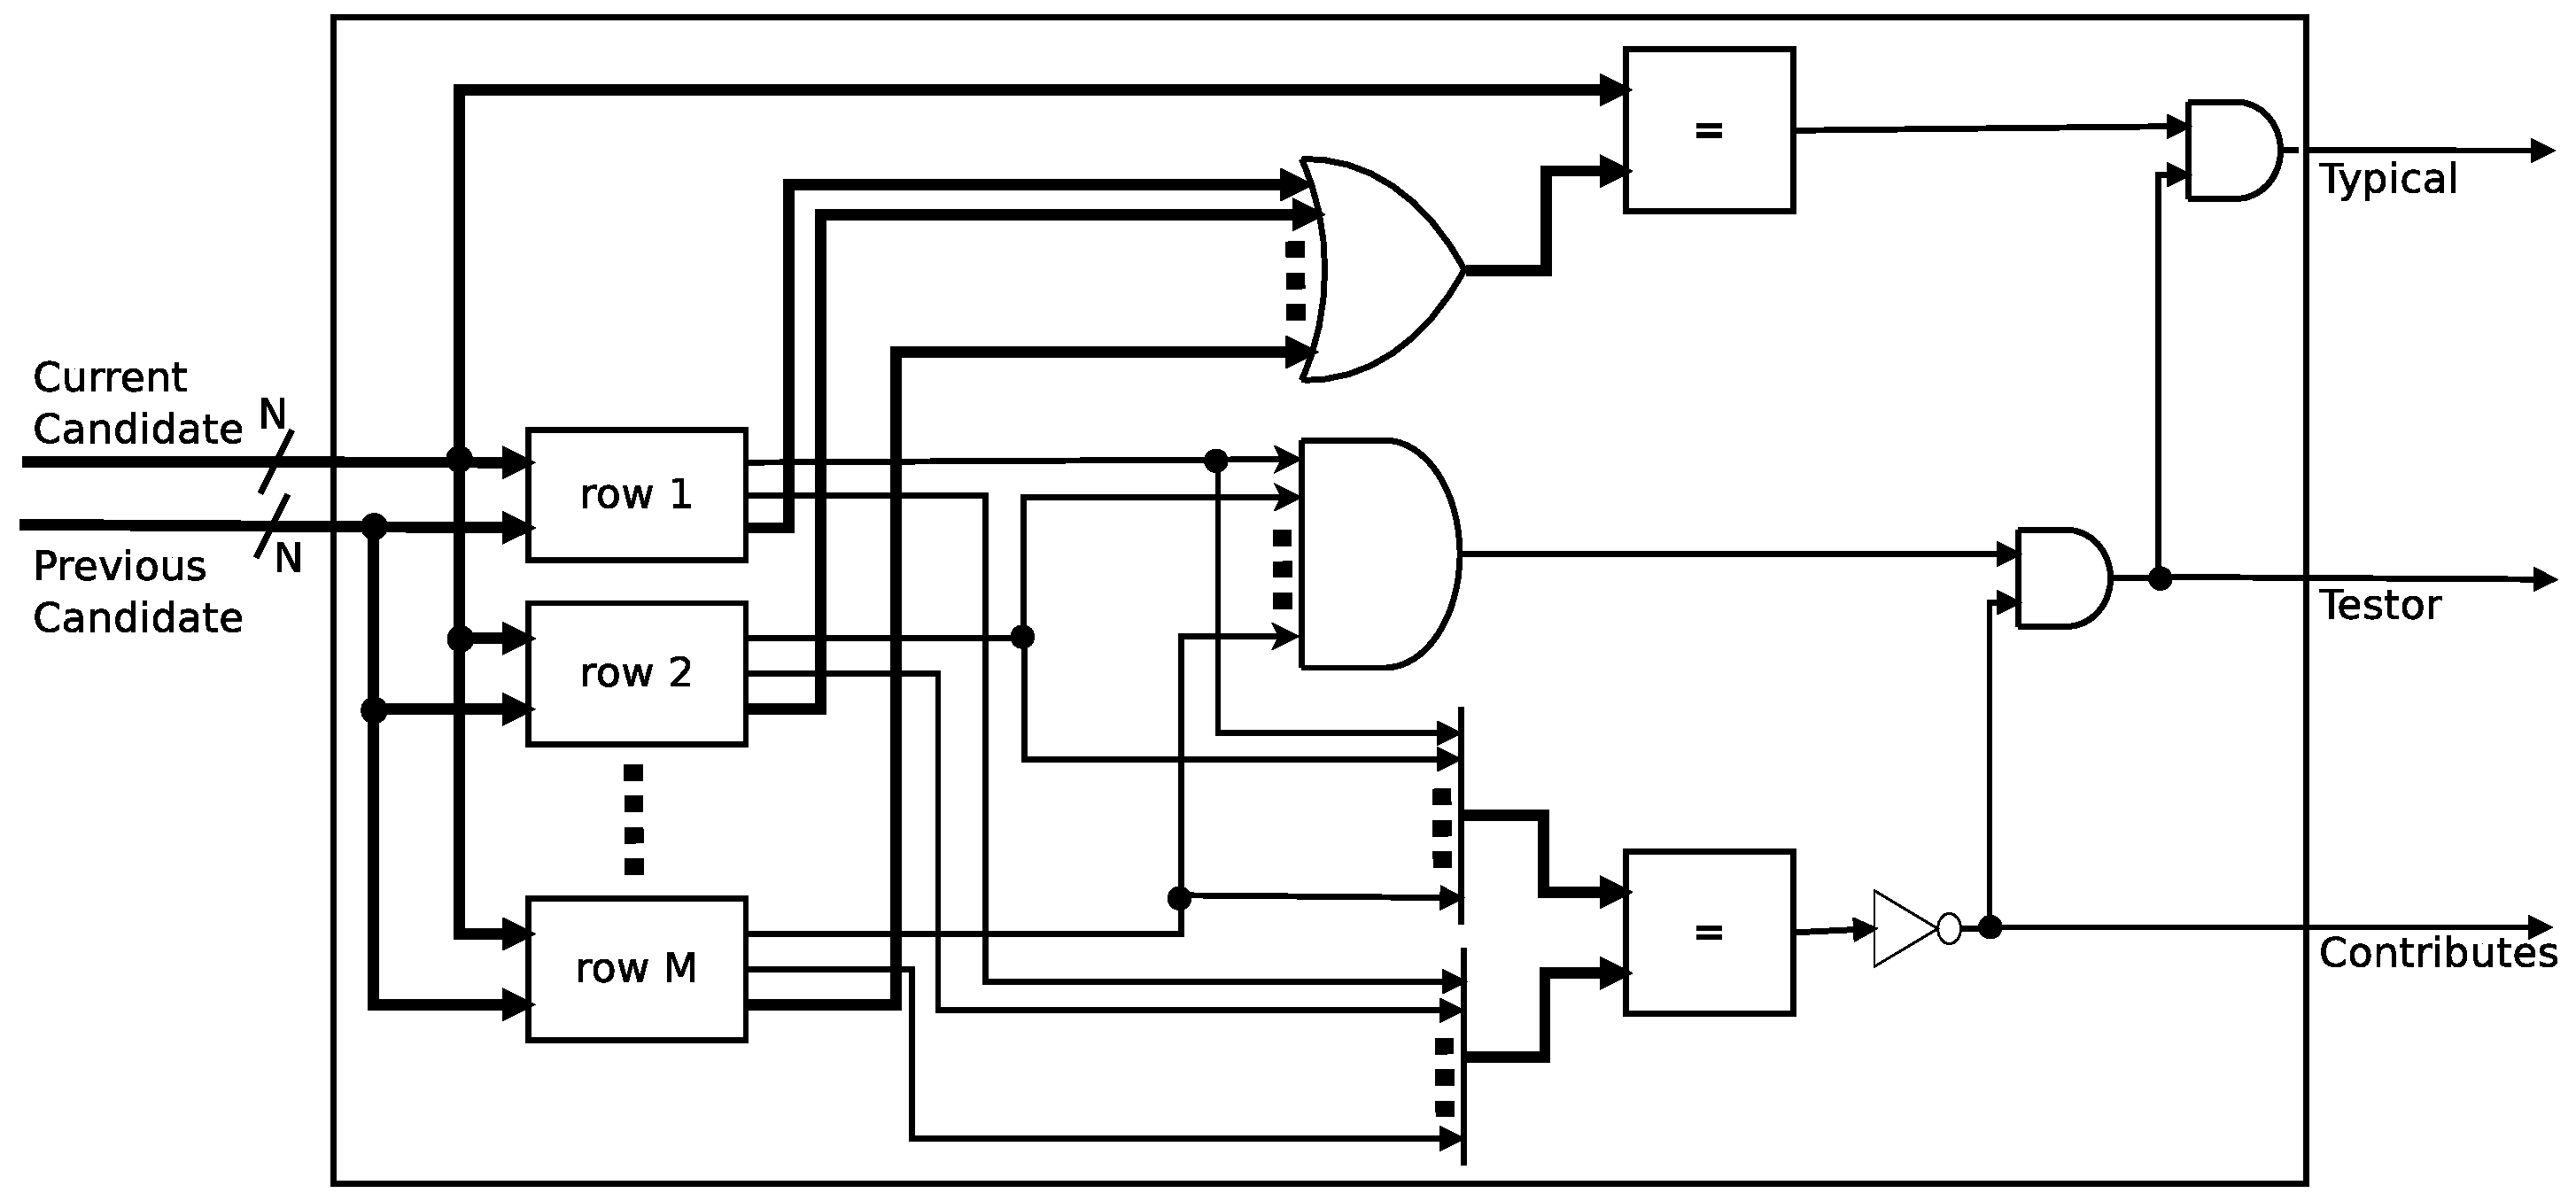
\includegraphics[height=6cm]{BM_module.eps}
    \end{center}
\caption{$BM$ module.}
\label{fig:4}
\end{figure}

The $BM$ module is composed of $M$ sub-modules named \textit{row~i}, as shown
in Fig.\,\ref{fig:4}. Each \textit{row~i} module contains a row ($n$ bits)
of the $BM$ matrix and the logic needed to perform a testor evaluation. To decide
whether an $n$-tuple is a testor, a bitwise AND operation is performed
between the value stored in each \textit{row~i} module and the current
candidate, as shown in Fig.\,\ref{fig:row}. If at least one bit of the AND operation is TRUE,
then the output \textit{Testor} of that particular \textit{row~i} sub-module
will be TRUE. The same operation is performed over the previous candidate.
If the output \textit{Testor} is different from
the output \textit{Contributes} for any \textit{row~i} sub-module,
it means that the current candidate reduces the amount of zero rows regarding the previous candidate and
then, the output \textit{Contributes} from the $BM$ module becomes TRUE.
If the output $Testor$ of all  \textit{row~i} sub-modules is
TRUE, then the output \textit{Testor} of the $BM$ module will be TRUE,
which means that the candidate is a testor of $BM$.


\begin{figure}[htb]
    \begin{center}
        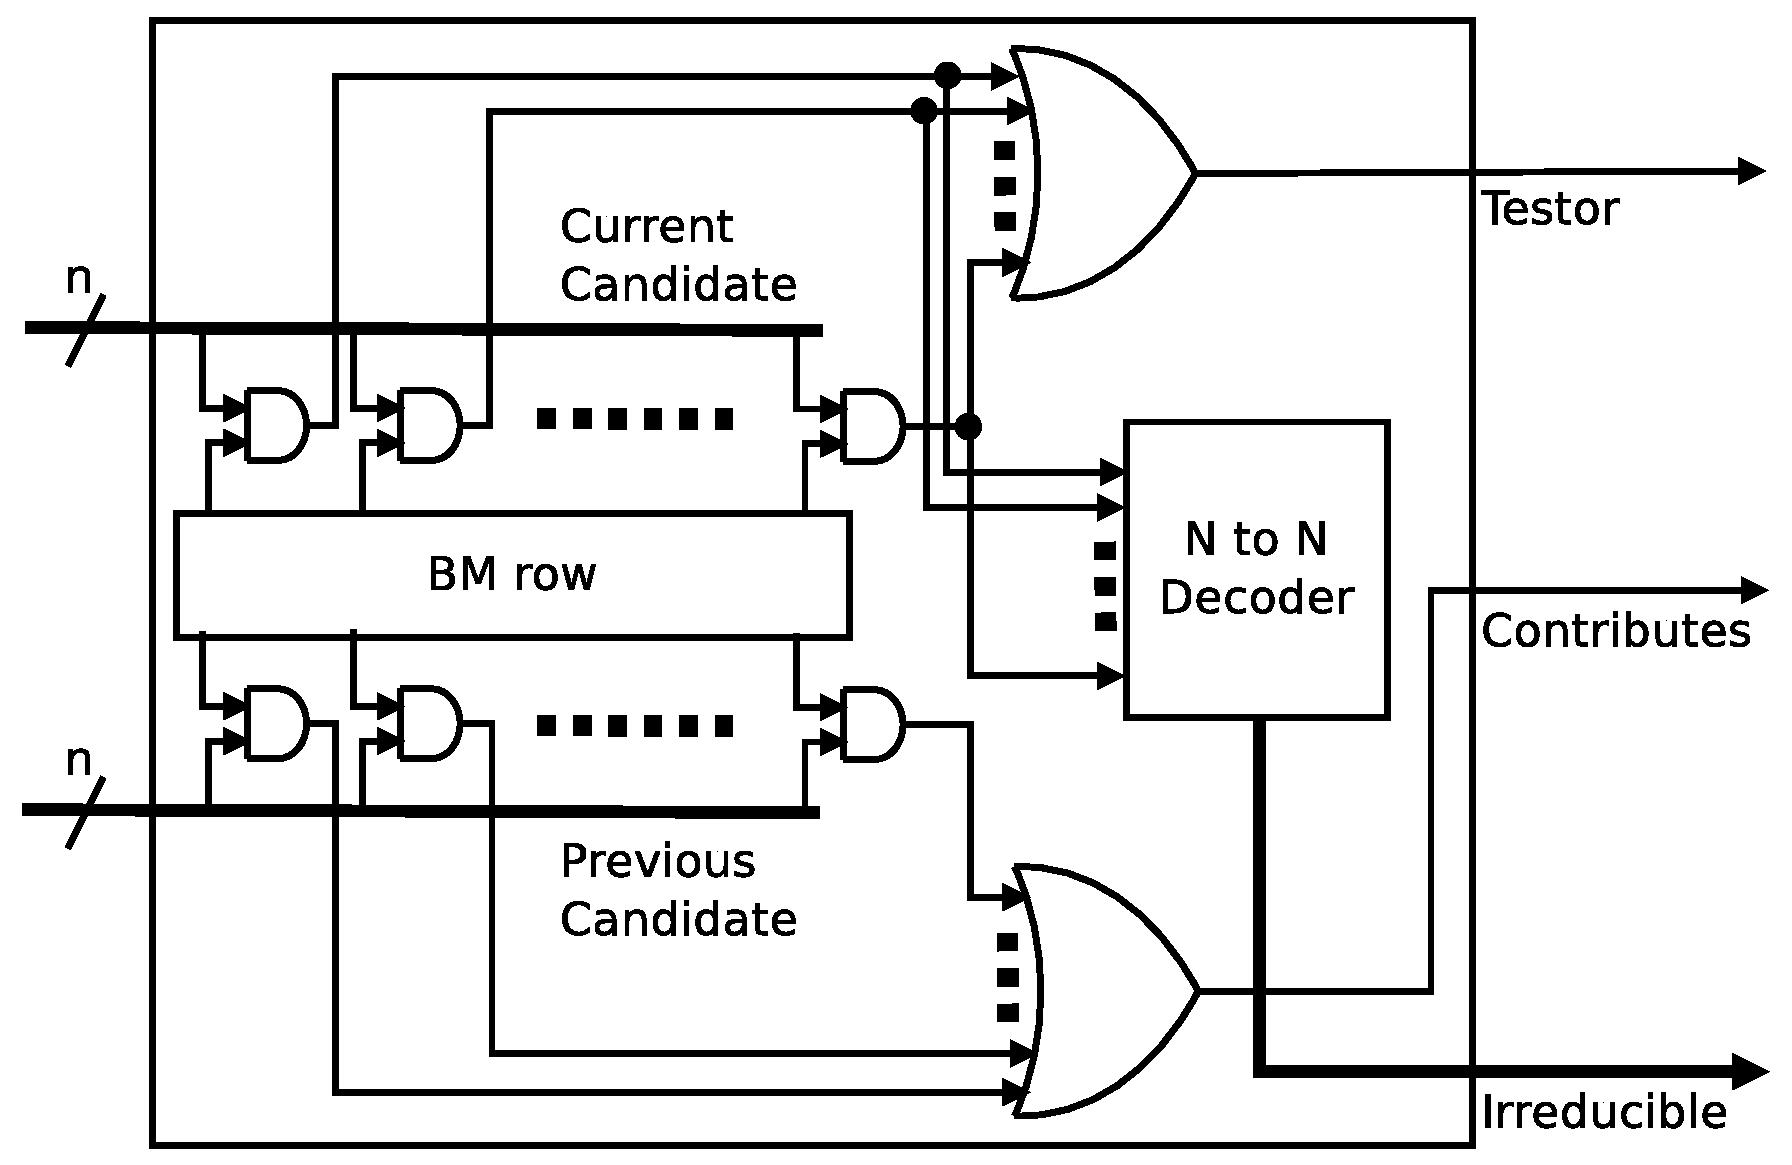
\includegraphics[height=6cm]{BM_row.eps}
    \end{center}
\caption{$BM$ row.}
\label{fig:row}
\end{figure}

In order to verify the irreducible condition, an \textit{N~to~N~Decoder}
receives as input the result of the AND operation between the current candidate and the corresponding $BM$ row.
The output from the \textit{N~to~N~Decoder} repeats the input when there is only one bit set
to 1, and returns zero otherwise. For those rows with only one bit having a 1 after ANDed with the candidate,
the attribute in the position of that bit is indispensable if the candidate is a testor.
According to definition~\ref{def24}, every attribute in a testor must be indispensable to be an
irreducible testor. %This idea is stated in definition~1 of \citep{R13}.

\setlength{\tabcolsep}{3pt}
\begin{table}[!htb]
    \begin{minipage}{.5\linewidth}
      \caption{An example of irreducible testor.}\label{table4}
      \centering
        \begin{tabular}{ ccccc|ccccc }
 			\hline                       
  			\multicolumn{5}{c|}{Cand. $\{x_0, x_1\}$} & 
  			\multicolumn{5}{c}{Decoder output} \\
  			\hline
			  $x_0$ &   $x_3$ &   $x_4$ &   $x_1$ &   $x_2$ &
  			  $x_0$ &   $x_3$ &   $x_4$ &   $x_1$ &   $x_2$ \\
  			\hline
  			1 & 0 & 0 & 0 & 0 & 1 & 0 & 0 & 0 & 0\\
  			0 & 0 & 0 & 1 & 0 & 0 & 0 & 0 & 1 & 0\\
  			1 & 0 & 0 & 1 & 0 & 0 & 0 & 0 & 0 & 0\\
  			\hline  
  			\multicolumn{5}{c|}{Candidate $=$} & 1 & 0 & 0 & 1 & 0\\
  			\hline  
		\end{tabular}
	%\end{table}
	%\begin{table}[!htb]
    \end{minipage}%
    \begin{minipage}{.5\linewidth}
      \centering
        \caption{An example of not irreducible testor.}\label{table5}
        \begin{tabular}{ ccccc|ccccc }
 			\hline                       
  			\multicolumn{5}{c|}{Cand. $\{x_0, x_4\}$} & 
  			\multicolumn{5}{c}{Decoder output} \\
  			\hline
  			%\multicolumn{5}{c|}{$x_0~x_3~x_4~x_1~x_2$}&\multicolumn{5}{c}{$x_0~x_3~x_4~x_1~x_2$}\\
  			  $x_0$ &   $x_3$ &   $x_4$ &   $x_1$ &   $x_2$ &
  			  $x_0$ &   $x_3$ &   $x_4$ &   $x_1$ &   $x_2$ \\
  			\hline
  			1 & 0 & 1 & 0 & 0 & 0 & 0 & 0 & 0 & 0\\
  			0 & 0 & 1 & 0 & 0 & 0 & 0 & 1 & 0 & 0\\
  			1 & 0 & 1 & 0 & 0 & 0 & 0 & 0 & 0 & 0\\
  			\hline  
  			\multicolumn{5}{c|}{Candidate $\neq$} & 0 & 0 & 1 & 0 & 0\\
  			\hline  
		\end{tabular}
    \end{minipage} 
\end{table}

Taking as example the ordered basic matrix of Table~\ref{table2}. In Table~\ref{table4} the irreducibility of  $\{x_0,x_1\}$ is evaluated while the same is done for $\{x_0,x_4\}$ in Table~\ref{table5}. Left rows show the result of the AND operation between each row of $BM$ and the candidate, while those rows in the right show the decoder output taking as input its corresponding left row. In the last row, the result of an OR operation over all above bits is shown. According to our previous explanation, the candidate $\{x_0,x_1\}$ is an irreducible testor given that the result of the OR operation is equal to the candidate itself; while candidate $\{x_0,x_4\}$ is not. This can be corroborated in Table~\ref{tab_example}.

\begin{figure}[t]
    \begin{center}
        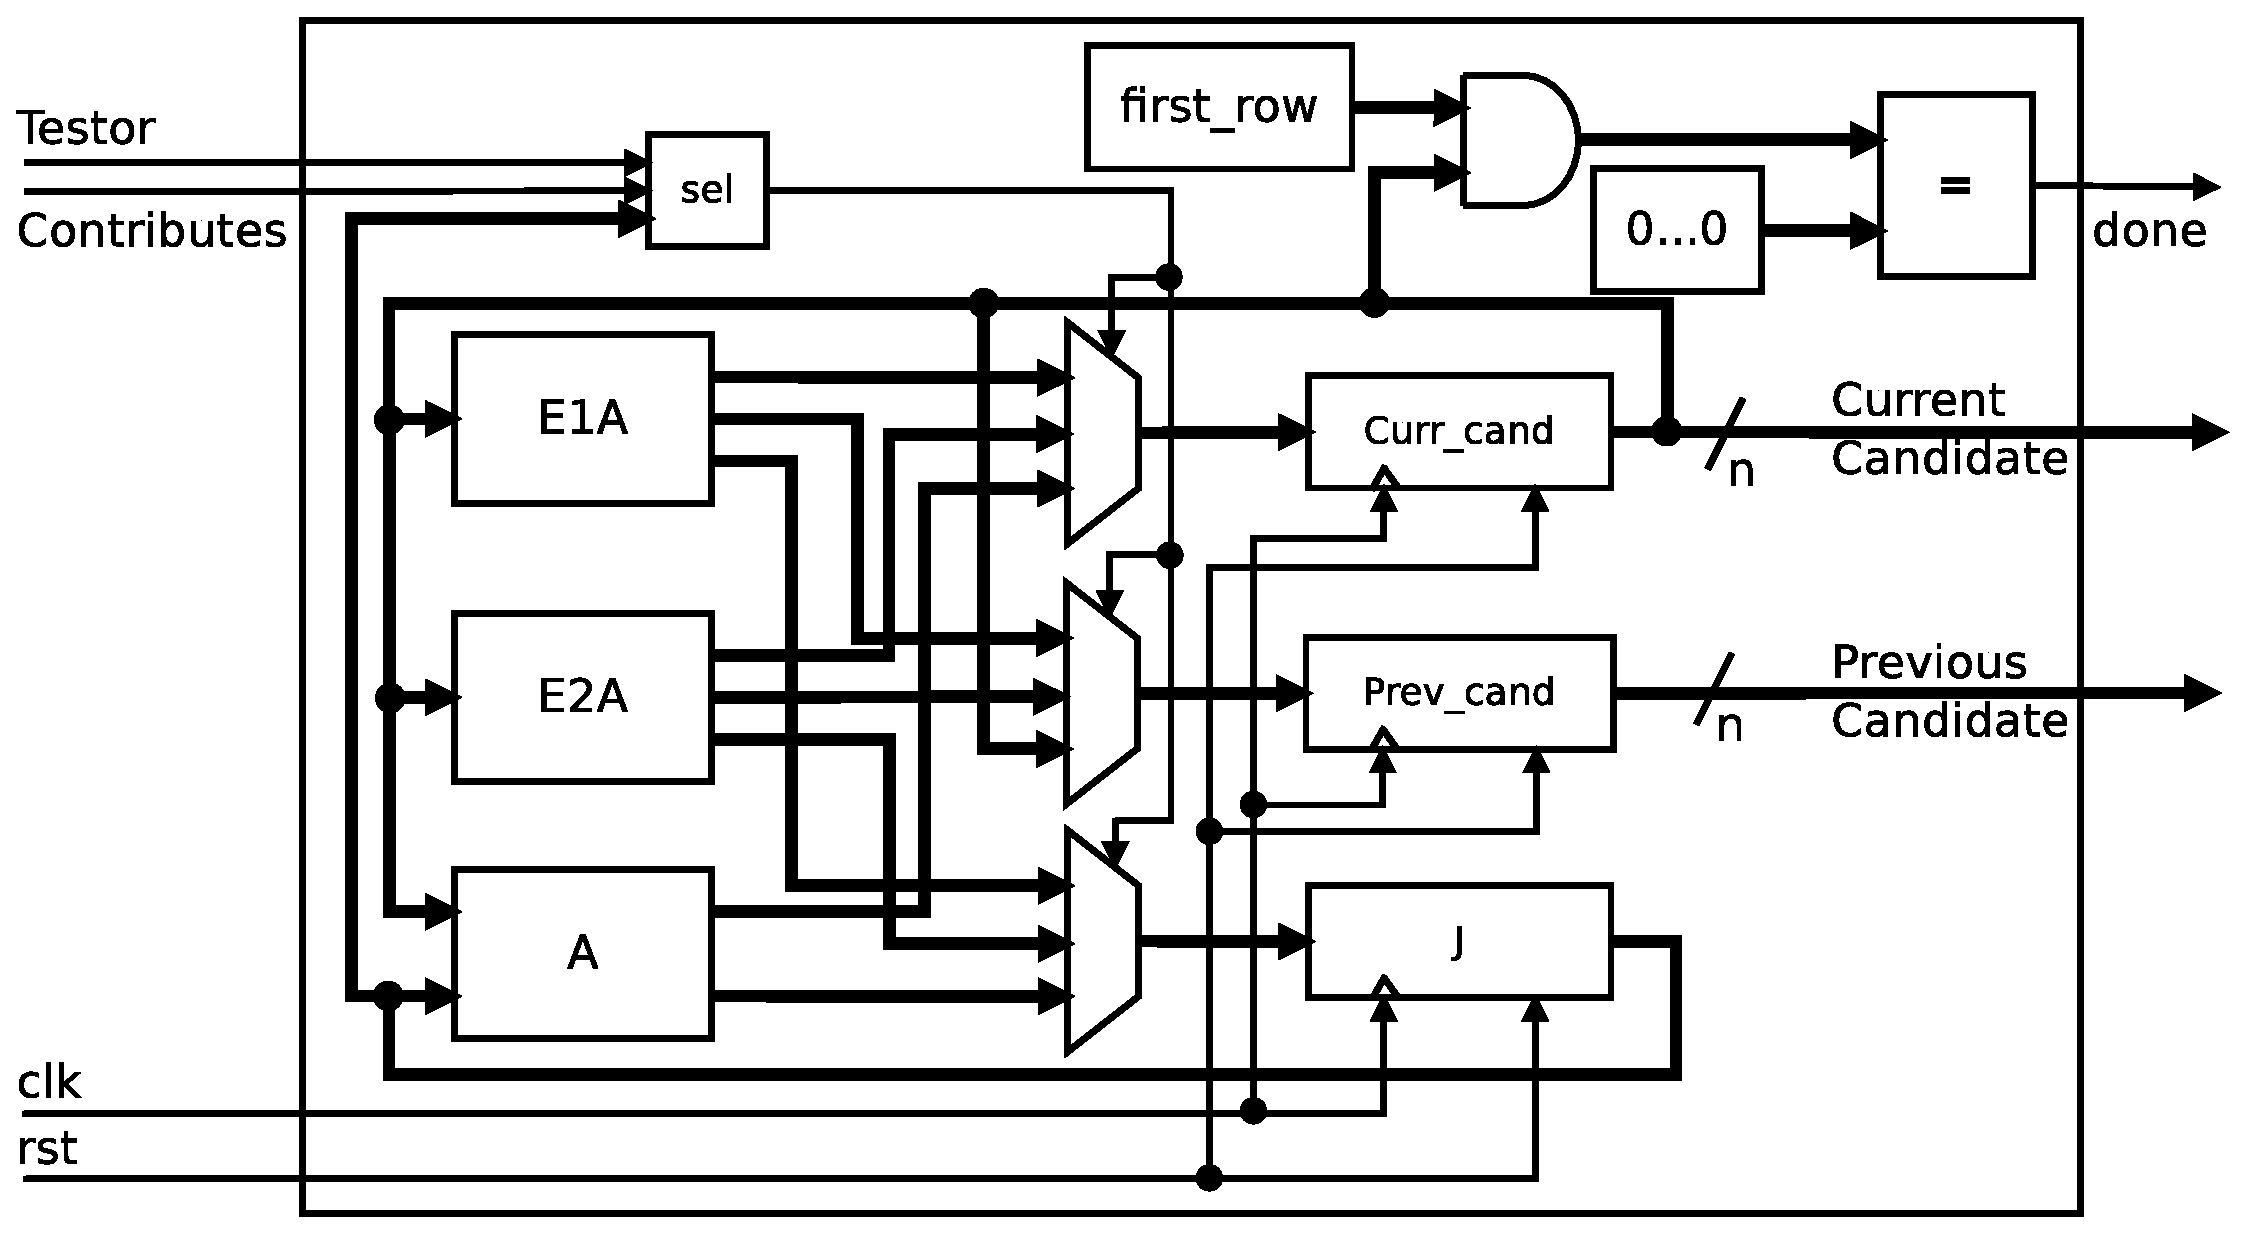
\includegraphics[height=6cm]{CandGen.eps}
    \end{center}
\caption{Candidate Generator module.}
\label{fig:5}
\end{figure}

The candidate generator module (Fig.\,\ref{fig:5}) uses the feedback from the $BM$ module
to calculate the next candidate to be evaluated. The
candidate generator module consists of three
registers for holding the current candidate (\textit{$Curr\_cand$}), the previous candidate
(\textit{$Prev\_cand$}) and the last added attribute ($J$). These registers values are updated
by the modules EA1, EA2 and A.

Depending on the combination of the input values, the outputs E1A,
E2A or A are used for updating the records. Table~\ref{tab_CandGen} shows how the records are updated 
according to the values of \textit{Testor}, \textit{Contributes} and $J$ inputs. 
This operation is computed by the module \textit{sel} shown in Fig.\,\ref{fig:5}.

 \begin{table}[htb]
		\caption{Candidate Generator Selector.} \label{tab_CandGen}
		\centering
 	\begin{tabular}{ccc}
 			\hline
 			Priority & Condition & Registers update\\
 			\hline
 			1 & \multicolumn{1}{>{\centering\arraybackslash}m{1in}}{$J=J_{max}$
 				($J_{max}=$ max value of $J$)} & \multicolumn{1}{>{\centering\arraybackslash}m{2in}}{
 				$Curr\_cand$ $\leftarrow$ E2A
 				$Prev\_cand$~$\leftarrow$~E2A
 				$J$~$\leftarrow$~E2A}\\
 			\hline
 			2 & \multicolumn{1}{>{\centering\arraybackslash}m{1.2in}}{Contributes $=0$ or Testor $=1$} &
 			\multicolumn{1}{>{\centering\arraybackslash}m{2in}}{
 				$Curr\_cand$ $\leftarrow$ E1A
 				$Prev\_cand$~$\leftarrow$~E1A
 				$J$~$\leftarrow$~E1A}\\
 			\hline
 			3 & \multicolumn{1}{>{\centering\arraybackslash}m{1.2in}}{Contributes $=1$ or Testor $=0$}&
 			\multicolumn{1}{>{\centering\arraybackslash}m{2in}}{
 				$Curr\_cand$ $\leftarrow$ A
 				$Prev\_cand$~$\leftarrow$~$Curr\_cand$
 				$J$~$\leftarrow$~A}\\
 			\hline       
 	\end{tabular}             
 \end{table}

The submodule $A$, shown in Fig.\,\ref{fig:subA}, assigns 1 to the next attribute at the right of 
the last bit with value 1 in the input candidate. The outputs of the submodule $A$ are the new candidate 
and $J+1$.

The submodule $E1A$, shown in Fig.\,\ref{fig:subEA1}, comprises the \textit{Rem$\_1$} 
(Fig.\,\ref{fig:subRem1}) and $A$ submodules. 
The submodule \textit{Rem$\_1$} deletes the last attribute added to the input candidate. 
This action is performed by a priority encoder which locates the last bit with value 1 in the input candidate. 
\textit{Rem$\_1$} outputs represent the previous candidate and the index of the deleted bit. 
%: $J$ and \textit{candidate} which is the input candidate without the last attribute. 
These outputs are connected to the corresponding inputs of the
submodule $A$, in order to add an attribute in the corresponding position. Finally, the outputs of $E1A$ 
represent the new candidate to be evaluated, the previous candidate and the index where the new attribute 
was added to the current candidate.

\begin{figure}[htb]
\centering
\begin{minipage}{.5\textwidth}
  \centering
   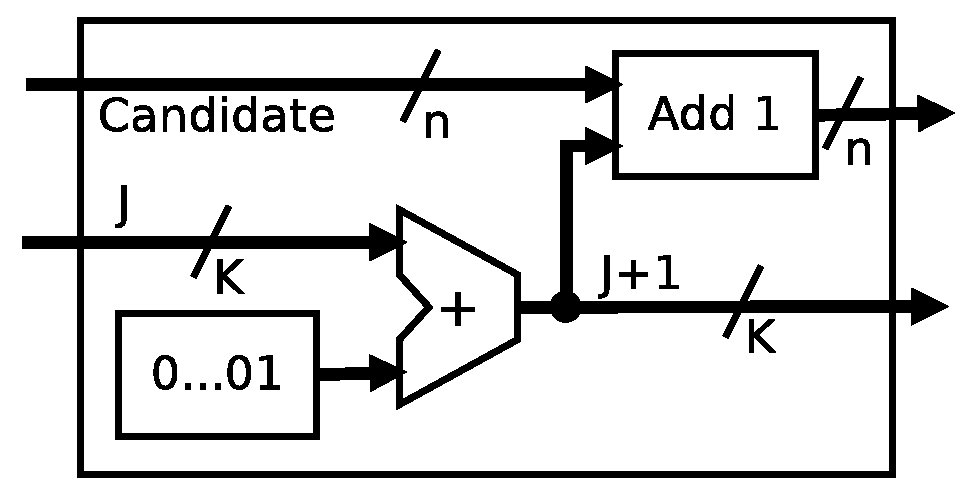
\includegraphics[width=.7\linewidth , height=3cm]{Add1.eps}
  \caption{Submodule A.}
  \label{fig:subA}
\end{minipage}%
\begin{minipage}{.5\textwidth}
  \centering
   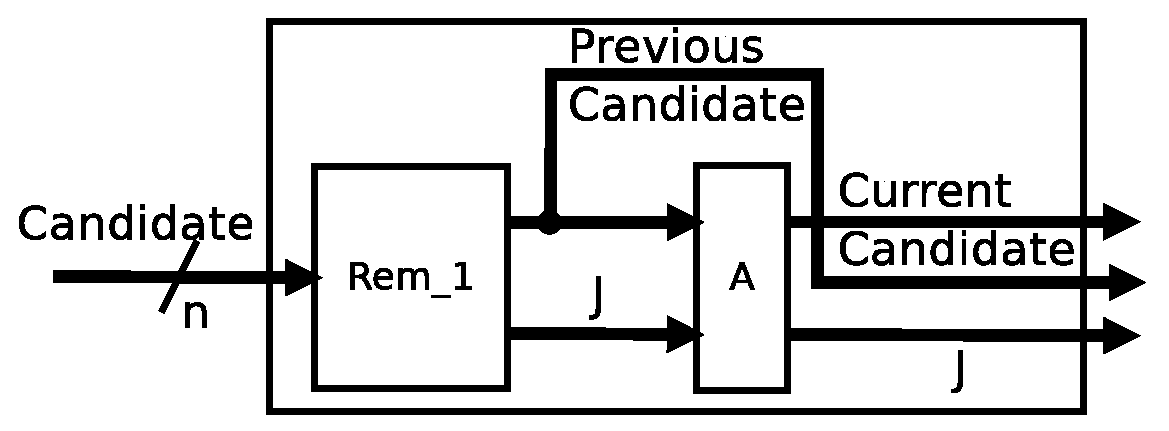
\includegraphics[width=\linewidth , height=3cm]{EA1.eps}
  \caption{Submodule E1A.}
  \label{fig:subEA1}
\end{minipage}
\end{figure}

Finally, the submodule $E2A$ removes the last two attributes from the
input candidate, and then adds the following corresponding attribute. This 
operation is performed by means of two \textit{Rem$\_1$} submodules and an $A$ submodule, as 
shown in Fig.\,\ref{fig:subEA2}.

In order to check if the execution of the CT-EXT  algorithm has finished, the result of an AND 
operation between the current candidate and the first row of the basic matrix is compared to 
the null $n$-tuple ($0,...,0$), as shown in the upper right corner of Fig.\,\ref{fig:5}. If the 
result of this comparison is TRUE, then the output $done$ is activated because any further 
candidate will not satisfy the testor condition over the first row of $BM$ 
(line~\ref{row1condition} of algorithm~\ref{ctext_algo}).

\begin{figure}[htb]
\centering
\begin{minipage}{.5\textwidth}
  \centering
   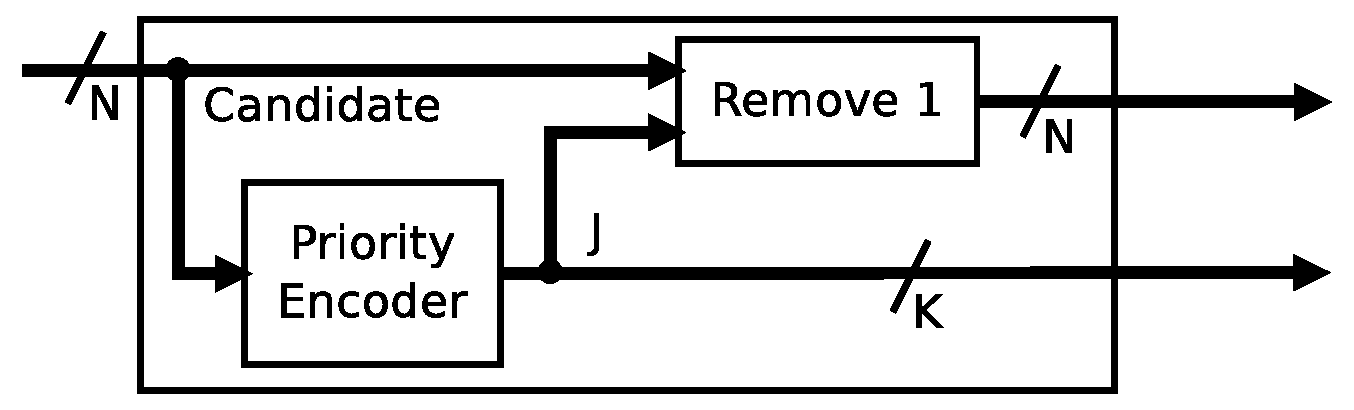
\includegraphics[width=\linewidth , height=3cm]{Rem1.eps}
  \caption{Submodule $Rem\_1$.}
  \label{fig:subRem1}
\end{minipage}%
\begin{minipage}{.5\textwidth}
  \centering
   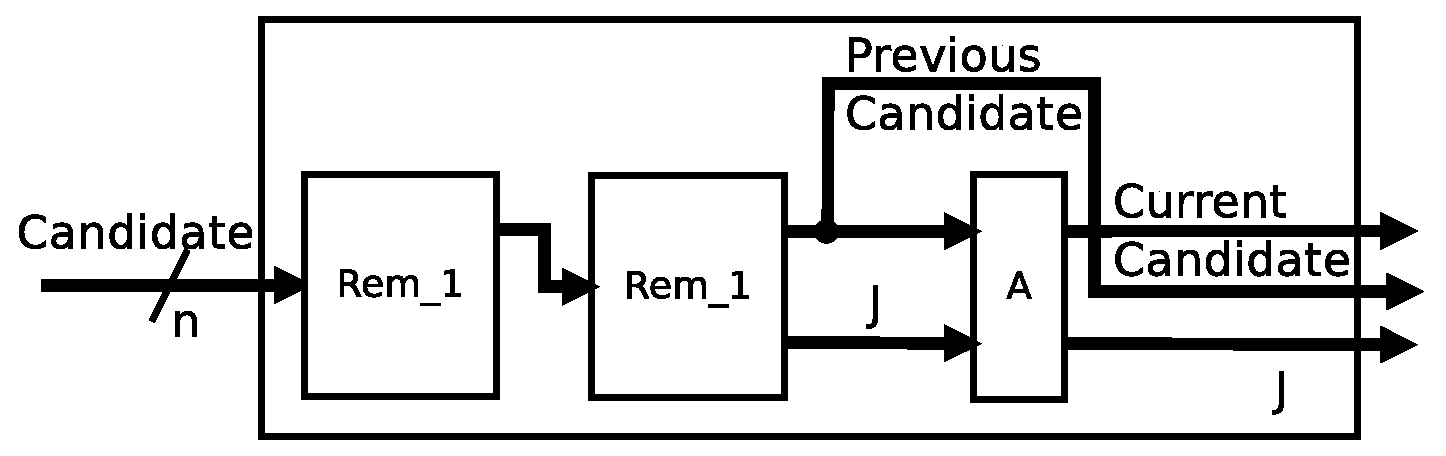
\includegraphics[width=\linewidth , height=3cm]{EA2.eps}
  \caption{Submodule E2A.}
  \label{fig:subEA2}
\end{minipage}
\end{figure}

\subsubsection*{The FPGA-based board}
The Atlys board from Digilent \citep{R15} was selected as the prototyping board. This board is 
a development and prototyping platform based on a Xilinx Spartan-6 LX45 FPGA, speed grade -3. The Atlys board 
supports device programming and simplified user-data transfer at a maximum rate of 48MB/s, over 
a single USB connection. 

The communication between the host PC and the FPGA uses the Digilent Synchronous 
Parallel Interface (DSTM) protocol \citep{R25}. Irreducible testors $n$-tuples, computed by the 
proposed architecture, are buffered within a FIFO in order to be split into bytes. These bytes 
are then buffered into a double clocked FIFO \citep{R26} to be read from the PC. This last FIFO 
ensures the output interface operation at 48MHz, as required by the DSTM protocol.

\subsection{Software Description}
\label{sect:5}

The software component allows the user to provide the basic matrix in a 
plain text file following the format shown in Fig.\,\ref{fig:8}. The software component is responsible for 
programming the FPGA device and communicating with the board during irreducible testor computation.

First, the basic matrix is reorganized by setting one of the rows with the minimum amount of ones as the 
first row and swapping columns in such a way those with a 1 in the first row appear on the left. 

Using the sorted basic matrix, a VHDL file is generated and the synthesis and optimization process is started.
This way, the optimization stage takes advantage of the basic matrix data to minimize the FPGA resource 
utilization. Then, the programming file for the FPGA device is generated.

On the running stage, the software component interacts with the hardware architecture. 
First, the device is programmed with the bit-file obtained from the previous stage. Then, the
hardware architecture starts computing irreducible testors. 
The software component keeps pulling through a USB port for new irreducible testors in the output 
FIFO until the $done$ signal is activated in the FPGA.

As a result of the sorting process, the order of attributes in the basic matrix is altered as can 
be seen comparing Tables~\ref{table1} and~\ref{table2}. Consequently, the irreducible testors calculated 
in the FPGA must be codified according to the order of columns in the original basic matrix. This task 
is performed by the software component and then the results are written to the output file.

\begin{figure}[t]
    \begin{center}
       \includegraphics[height=2.8cm]{infile.eps}
    \end{center}
\caption{Input file format.}
\label{fig:8}
\end{figure}

\section{Evaluation and Discussion}
\label{sect:6}


In order to show the performance of the proposed platform, it was compared against a software 
implementation of the CT-EXT algorithm~\citep{R22} and the BT hardware platform previously 
reported in~\citep{Rod14}\footnote{The source code of the three implementations and the basic matrix
generator, as well as the matrices used for the experiments, can be downloaded from 
\textbf{http://ccc.inaoep.mx/}.} .
 
%For experimentation purposes, the BT hardware platform was modified for finding irreducible testors 
%on the FPGA similarly to the CT-EXT implementation. This modification avoids the final filtering stage 
%proposed by \cite{R21}.

Either CT-EXT or BT hardware implementations are capable of evaluating a candidate per clock 
cycle. If both architectures are running at the same frequency, as it will be the case in our experiments, 
there are two reasons for differences in running time. The first one is the time taken for reorganization 
of basic matrix, which is a more complex process in BT, altough it can be neglected as shown in \citep{R21}. 
The second and the most relevant, is the amount of candidates to be evaluated. 
%It is not a difficult task to find a $BM$ in which BT evaluates less candidates than CT-EXT or vice versa.

Regarding to the software implementation, the CT-EXT hardware platform has two disadvantages. First, 
VHDL code is generated for each $BM$ data and a process of synthesis must be executed previously to 
executing the algorithm; while this is unnecessary in the software version of CT-EXT. Secondly, the 
software will be running in a PC at a frequency of 3.10GHz while FPGA architecture will run at 50MHz. 

These disadvantages make the hardware approach useful (faster) under two conditions. First, the number of 
candidates to be evaluated is big enough to overcome the synthesis overhead. Second, the dimensions of the 
$BM$ are big enough to provide a considerable speed up of the candidate evaluation process. Although 
the hardware architecture could be designed for a fixed maximum matrix size and receive the $BM$ through the 
USB port, by doing this, the size of the problem which can be solved would be significantly reduced. The 
synthesis process comprehend an optimization of the design, taking advantage of the $BM$ data distribution for 
the reduction of the generated hardware configuration. The number of operations for the evaluation of a single 
candidate, in the software approach, is proportional to the number of rows and it is directly related to the 
number of columns in the $BM$. Using this approach it is possible to achive a significant reduction in the processing time, even if
operating at a much lower clock frequency, by evaluating a candidate on each clock cycle.

With these points in mind and in order to show the usability of the proposed platform, 
three kinds of basic matrices were randomly generated. Each type containing different percentage of 1's: 
\begin{enumerate}
	\item Very-low density matrices: approximately 8\%.
	\item Low density matrices: approximately 33\%.
	\item Medium density matrices: approximately 45\%.
\end{enumerate}

Higher density matrices were discarded because they do not constitute a computationally expensive problem, 
as stated by \cite{R21}. Here after, we will be referring to these three sets of matrices by its 
approximate density of~1's.

\begin{figure}[htb]
\centering
\begin{minipage}{.5\textwidth}
  \centering
   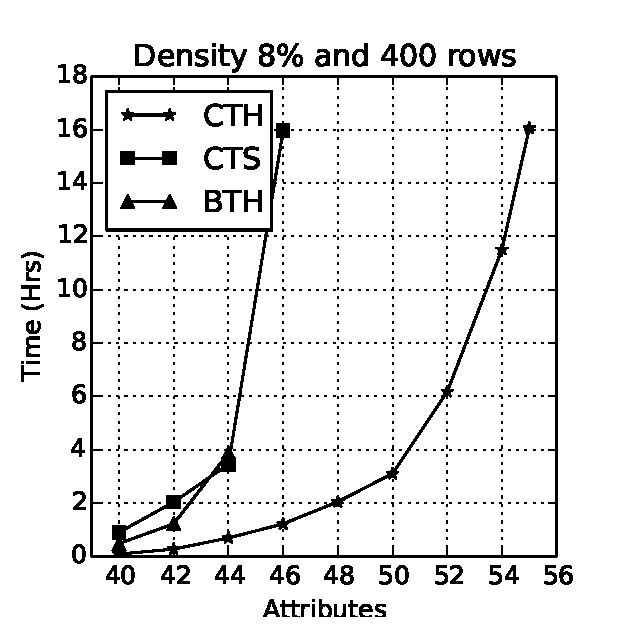
\includegraphics[width=\linewidth , height=5.5cm]{low_density.eps}
  \caption{Total runtime for density 8\%.}
  \label{fig:result1}
\end{minipage}%
\begin{minipage}{.5\textwidth}
  \centering
   \includegraphics[width=\linewidth , height=5.5cm]{med_density.eps}
  \caption{Total runtime for density 33\%.}
  \label{fig:result2}
\end{minipage}
\end{figure}

\begin{figure}[htb]
    \begin{center}
       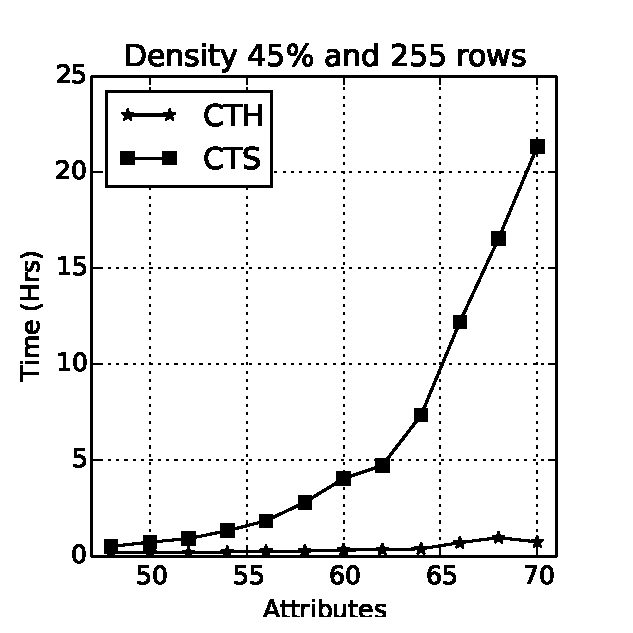
\includegraphics[height=5.5cm]{med48_density.eps}
    \end{center}
\caption{Total runtime for density 45\%.}
\label{fig:result3}
\end{figure}

For our experiments, 28 basic matrices of different sizes were randomly generated. 
A random number generator is used to generate rows up to 30 attributes long. The generated number is 
filtered for the minimum and maximum number of 1's allowed. This way the desires density is
controlled. If accepted, the row is verified as typical against the saved rows. Typical rows 
are saved until the desired number is reached. In order to obtain matrices with a larger
number of attributes, columns from different matrices are jointed. Finally the resulting 
density of 1's is calculated.

For the hardware platforms, we measure the runtimes including the time for the following stages: $BM$ input parsing 
and VHDL code generation, synthesis process, and irreducible testor computation (with the hardware 
component running at 50MHz). The number of rows for each type of matrices is conditioned by the dimensions of 
the biggest matrix that may be synthesized at the desired running frequency.
All experiments are performed using an Intel(R) Core(TM) i5-2400 CPU @ 3.10GHz for software executions and 
an Atlys board, powered by a Spartan-6 LX45 FPGA device, for the hardware components.
Figs.\,\ref{fig:result1}, \,\ref{fig:result2}, and \,\ref{fig:result3} show graphs of the runtime (in hours) 
for the three types of basic matrices. 

The proposed CT-EXT hardware platform (CTH) results were taken as reference for axis limits in 
Figs.\,\ref{fig:result1}, \,\ref{fig:result2}, and \,\ref{fig:result3}.
Slowest executions of the CT-EXT software implementation (CTS) are not shown in order to keep clarity in 
the figures. 
The hardware platform for BT (BTH) was not able to met the constrain of 50MHz clock frequency for some 
matrices. In fact, for medium  density, BT platform could not be synthesized even for the smallest matrix. 
This is the case for all missing BTH executions in Figs.\,\ref{fig:result1},~\,\ref{fig:result2}, and~\,\ref{fig:result3}.

\cite{R21} stated that the time for computing irreducible testors does not only depend on the size and 
density of the $BM$, but also on the distribution of 0's and 1's inside the matrix. This assertion can 
be also confirmed from matrices with 68 and 70 attributes respectively, in Fig.\,\ref{fig:result3}.

Table~\ref{table:8} shows the runtime for each stage of the data flow, for 
400x40, 400x42 and 400x44 very-low density matrices. This table shows that the synthesis time 
becomes less significative regarding the total time when the problem size increases. 
From this table, it can also be seen that the main difference between the BT and CT-EXT hardware 
implementations is the runtime of the irreducible testor computation process. The main reason for 
this difference is the number of candidates evaluated by each algorithm. This is an explanation 
about why the BT hardware implementation is slower than the software version of CT-EXT for the 
largest matrix in Table~\ref{table:8}.


\begin{table}[htb]
\caption{Processing time in seconds (broken down for each stage) for 
400x40, 400x42 and 400x44 very-low density matrices.} \label{table:8}
\begin{center}
    \begin{tabular}{lcccccc}   \hline
    	   Dimensions                & \multicolumn{2}{c}{400x40} & \multicolumn{2}{c}{400x42} 
    	                             & \multicolumn{2}{c}{400x44} \\ \hline
    	    	Stage	        			& CTH & BTH	& CTH & BTH & CTH & BTH \\ \hline
    	    Load and file generation & 0.05& 0.07& 0.05& 0.06& 0.06& 0.06\\
    	    Synthesis process        & 253 & 656 & 401 & 564 & 452 & 612\\
    	    Algorithm execution      & 300 & 1071& 970 & 3826& 2031& 13311\\ \hline
    	    Total time               & 554 & 1727& 1372& 4390& 2484& 13924\\ \hline
    	    CTS total time               & \multicolumn{2}{c}{3238} & \multicolumn{2}{c}{7320} 
    	    								& \multicolumn{2}{c}{12420}\\ \hline
    	    
    \end{tabular}
\end{center}
\end{table}

Tables~\ref{table:6} and~\ref{table:7} summarize the FPGA resource utilization on our prototyping board. 
The maximum operation frequency from Tables~\ref{table:6} and~\ref{table:7} shows that usually the CT-EXT 
implementation is potentially faster than the modified BT implementation. Resource utilization is 
directly related to $BM$ dimensions, its density and to a lesser extent to data organization.

\begin{table}[htb]
\caption{Synthesis summary of resource utilization for $BM$ with 8\% density on an Spartan-6 LX45 
FPGA device.} \label{table:6}
\begin{center}
    \begin{tabular}{lcccc}   \hline
    	    Dimensions & \multicolumn{2}{c}{400x40} & \multicolumn{2}{c}{400x44} \\ \hline
    	    Algorithm & BT & CT-EXT & BT & CT-EXT \\ \hline
        Slices & 1,398 (20\%) & 983 (14\%) & 1,554 (22\%) & 1,209 (17\%)  \\
        6-input LUTs & 4,010 (14\%) & 2,806 (10\%)& 4,475 (16\%)  & 3,004 (11\%)\\
        Flip-Flops & 832 (1\%) & 852 (1\%) & 876 (1\%) & 938 (1\%)\\
        Max clock freq & 80.44MHz & 179.58MHz & 84.56MHz & 173.24MHz\\ \hline
    \end{tabular}
\end{center}
\end{table}

\begin{table}[htb]
\caption{Synthesis summary of resource utilization for $BM$ with 33\% density on an Spartan-6 LX45 
FPGA device.} \label{table:7}
\begin{center}
    \begin{tabular}{lcccc}   \hline
    	    Dimensions & \multicolumn{2}{c}{225x50} & \multicolumn{2}{c}{225x55} \\ \hline
    	    Algorithm & BT & CT-EXT & BT & CT-EXT \\ \hline 
        Slices & 1,381 (20\%) & 1,554 (22\%) & 1,455 (21\%) & 1,562 (22\%) \\
        6-input LUTs & 3,769 (13\%) & 4,315 (15\%) & 4,135 (15\%) & 5,026 (18\%)\\
        Flip-Flops & 949 (1\%) & 980 (1\%) & 1,002 (1\%) & 1,039 (1\%)\\
        Max clock freq & 87.46MHz & 155.40MHz & 85.27MHz & 156.35MHz\\ \hline
    \end{tabular}
\end{center}
\end{table}

%\section{Discussion}
%\label{sect:7}

As it was shown in the previous section, the proposed hardware platform provides higher processing
performance than the software implementation of the CT-EXT
algorithm for the matrices used in our experimentation. 
This behaviour is possible because the hardware
component of the proposed platform is capable of testing whether a 
candidate is a testor of a $BM$ in a single clock cycle,
independently of the number of columns and rows, whereas
the software implementation runtime will significantly
increase for matrices with a large number of rows.

Experiment results show that the proposed platform beats the software implementation of
the CT-EXT algorithm, with ratios of around \textbf{one order} of magnitude. However, for large 
enough datasets this improvement could be significantly higher, as can be inferred from 
Fig.\,\ref{fig:result3}.

\section{Conclusions}
\label{sect:8}
In this work we present the design and implementation of a new hardware software platform for
computing all the irreducible testors in a dataset.  As opposed to the existing hardware 
architectures for feature selection using rough sets methods, our proposal computes all the
minimal subsets of features that preserve the classification accuracy of the original dataset.
The good performance of our hardware implementation, compared to the software approach, is 
feasible due to the high level of parallelism implicit in candidates evaluation of the CT-EXT 
algorithm; which can be efficiently implemented on an FPGA. 
%The proposed platform improves the previously reported architecture \citep{R21} by finding 
%\textit{irreducible} testors in a single clock cycle. This new feature solves problems arising 
%from transmission of irrelevant data to the hosting PC; improving the total runtime. 
This proposed architecture offers an alternative to the hardware implementation of BT which is 
faster in most of the cases, by evaluating less candidate subsets. 

Experiments also showed that the proposed platform uses fewer hardware resources and is able to run at a higher 
frequency than the BT hardware implementation, which allows processing larger matrices, since the maximum size of 
the problem that can be solved in a hardware architecture is conditioned by its resource utilization. 
This work enables the application of Testor Theory methods in larger classification and decision-making
problems than it was possible.

The search for new algorithms that could be efficiently implemented in an FPGA constitutes future work. Improvements, such as testing two or more candidates per iteration, are still unexplored and would be 
evaluated in further studies.



%\section*{References}
\bibliographystyle{elsarticle-harv}


%% References without bibTeX database:

\begin{thebibliography}{00}

\bibitem[Compton et al.(2002)]{R29}Compton, K., and Hauck, S. (2002). Reconfigurable computing: a survey of systems and software. ACM Computing Surveys (csuR), 34(2), 171-210.
\bibitem[Cumplido et al.(2006)]{R10} Cumplido, R., Carrasco, A. and Feregrino, C. (2006). On the Design and Implementation of a High Performance Configurable Architecture for Testor Identification. Lectures Notes on Computer Science, 4225, 665-673.
\bibitem[Djukova(2005)]{R8}Djukova, E. V. (2005). On the number of irreducible coverings of an integer Matrix. Computational Mathematics and Mathematical Physics, 45, 903-908.
\bibitem[Dmitriev et al.(1966)]{R12} Dmitriev, A. N.,  Zhuravlev, Y. I. and Krendeliev, F. P. (1966). About Mathematical Principles of Objects and Phenomena Classification. Diskretni Analiz, 7, 3-17.
\bibitem[G\'omez(2001)]{R16}G\'omez, M. (2001). Hardware-in-the-Loop Simulation. Embedded Systems Programming, 14, 38-49.

\bibitem[Grze et al.(2013)]{Grze13}Grze, T., Kopczynski, M., Stepaniuk, J. (2013). FPGA in Rough Set Based Core and Reduct Computation. In Rough Sets and Knowledge Technology, 263-270.

\bibitem[Guyon et al.(2003)]{R4}Guyon, I. and Elisseeff, A. (2003). An introduction to variable and feature selection. Journal of Machine Learning Research, 3, 1157-1182.
\bibitem[Jain et al.(1997)]{R3}Jain, A. and Zongker, D. (1997). Feature Selection: Evaluation, Application, and Small Sample Performance. IEEE Transactions on Pattern Analysis and Machine Intelligence, 9, 153-158.

\bibitem[Jensen and Shen (2014)]{Jensen14}Jensen, R., Tuson, A., Shen, Q. (2014). Finding rough and fuzzy-rough set reducts with SAT. Information Sciences, 255, 100-120.

\bibitem[Kopczynski et al.(2014)]{Kop14}Kopczynski, M., Grze, T., Stepaniuk, J. (2014). FPGA in Rough-Granular Computing : Reduct Generation. In 2014 IEEE/WIC/ACM International Joint Conferences on Web Intelligence (WI) and Intelligent Agent Technologies (IAT), 364-370. 

\bibitem[Kudryavtsev(2006)]{R9}Kudryavtsev, V. B. (2006). Test recognition theory. Discrete Applied Mathematics, 16, 319-350.
\bibitem[Lazo-Cort\'es et al.(1995)]{R32}Lazo-Cort\'es, M., Ruiz-shulcloper, J. (1995). Determining the feature relevance for non-classically described objects and a new algorithm to compute typical fuzzy testors. Pattern Recognition Letters, 16(12), 1259-1265.
\bibitem[Lazo-Cort\'es et al.(2001)]{R1}Lazo-Cort\'es, M., Ruiz-shulcloper, J., and Alba-cabrera, E. (2001). An Overview of the Evolution of the Concept of Testor. Pattern Recognition, 34, 753-762.

\bibitem[Lazo-Cort\'es et al.(2015)]{Lazo15}Lazo-Cortés, M. S., Mart\'inez-Trinidad, J. F., Carrasco-Ochoa, J. A. and Sanchez-D\'iaz, G. (2015). On the relation between rough set reducts and typical testors. Information Sciences, 294, 152-163.

\bibitem[Mart\'inez et al.(2007)]{Mart07}Mart\'inez, N., Le\'on, M. and Garc\'ia, Z. (2007). Features selection through FS-testors in case-based systems of teaching-learning. In MICAI 2007: Advances in Artificial Intelligence, 1206-1217.

\bibitem[Mart\'inez-Trinidad et al.(2001)]{R5}Mart\'inez-Trinidad, J.F. and Guzm\'an-Arenas, A. (2001). The Logical Combinatorial Approach to Pattern Recognition an Overview through Selected Works. Pattern Recognition, 34, 741-751.

\bibitem[Medina et al.(2007)]{Med07}Medina, D., Mart\'inez, N., Garc\'ia, Z., Ch\'avez, M. and Garc\'ia, M. (2007). Putting Artificial Intelligence Techniques into a Concept Map to Build Educational Tools. In Nature Inspired Problem-Solving Methods in Knowledge Engineering, 617-627.

\bibitem[Pocek et al.(2013)]{R30}Pocek, K., Tessier, R. and DeHon, A. (2013). Birth and adolescence of reconfigurable computing: A survey of the first 20 years of field-programmable custom computing machines. In Highlights of the First Twenty Years of the IEEE International Symposium on Field-Programmable Custom Computing Machines (pp. 3-19).

\bibitem[Rodr\'iguez et al.(2014)]{Rod14} Rodr\'iguez, V., Mart\'inez, J. F., Carrasco, J. A., Lazo, M. S., Cumplido, R. and Feregrino-Uribe, C. (2014). A hardware architecture for filtering irreducible testors. In ReConFigurable Computing and FPGAs (ReConFig), 2014 International Conference on, 1-4.

\bibitem[Rojas et al.(2007)]{R11}Rojas, A., Cumplido, R., Carrasco-Ochoa, J. A., Feregrino, C. and Mart\'inez-Trinidad, J. f. (2007). FPGA Based Architecture for Computing Testors. Lectures Notes on Computer Science, 4881, 188-197.
\bibitem[Rojas et al.(2012)]{R21}Rojas, A., Cumplido, R., Carrasco-Ochoa, J. A., Feregrino, C. and Mart\'inez-Trinidad, J. f. (2012). Hardware-software platform for computing irreducible testors. Expert Systems with Applications, 39, 2203 - 2210.
\bibitem[Ruiz-Shulcloper et al.(1985)]{R31}Ruiz-Shulcloper, J., Aguila-Feros, L. and Bravo-Mart\'inez, A. (1985). BT and TB algorithms for computing all irreducible testors. Revista Ciencias Matem\'aticas, 2, 11-18.
\bibitem[Ruiz-Shulcloper(2008)]{R27}Ruiz-Shulcloper, J. (2008). Pattern recognition with mixed and incomplete data. Pattern Recognition and Image Analysis, 18(4), 563-576.
\bibitem[S\'anchez-D\'iaz et al.(2002)]{R13}S\'anchez-D\'iaz, G. and Lazo-Cort\'es, M. (2002). Modifying BT Algorithm for Improving its Runtimes. Revista Ciencias Matem\'aticas, 20, 129-136.
\bibitem[S\'anchez-D\'iaz et al.(2007)]{R22}S\'anchez-D\'iaz, G. and Lazo-Cort\'es, M. (2007). CT-EXT: An Algorithm for Computing Typical Testor Set. Lecture Notes in Computer Science, 4756, 506-514.
\bibitem[S\'anchez-D\'iaz et al.(2010)]{R23}S\'anchez-D\'iaz, G., Piza-Davila, I, Lazo-Cort\'es, M, 
Mora-Gonz\'alez, M and Salinas-Luna, J. (2010). A Fast Implementation of the CT-EXT Algorithm for the Testor Property Identification. Lecture Notes in Computer Science, 6438, 92-103.
\bibitem[Skowron et al.(1992)]{R40}Skowron, A and Rauszer, C. (1992). The discernibility matrices and functions in information systems. Handbook of Applications and Advances of the Rough Sets Theory, 331-362.

\bibitem[Tiwari et al.(2013)]{Tiwari13}Tiwari, K., Kothari, A., Shah, R. (2013). FPGA Implementation of a Reduct Generation Algorithm based on Rough Set Theory. International Journal of Advanced Electrical and Electronics Engineering (IJAEEE), 2(6), 55-61.

\bibitem[Tiwari and Kothari (2013)]{Tiwari14} Tiwari, K., Kothari, A. (2014). Design and Implementation of Rough Set Algorithms on FPGA : A Survey, 3(9), 14-23.

\bibitem[Torres et al.(2014)]{Torr14}Torres, M., Torres, A., Cuellar, F., Torres, M., Ponce de Le\'on, E. and Pinales, F. (2014). Evolutionary computation in the identification of risk factors. Case of TRALI. Expert Systems with Applications, 41(3), 831-840.

\bibitem[Yahia et al.(2000)]{Yah00}Yahia, M. E., Mahmod, R., Sulaiman, N. and Ahmad, F. (2000). Rough neural expert systems. Expert Systems with Applications, 18(2), 87-99.

\bibitem[Digilent(2013)]{R15}Atlys Board Reference Manual. Digilent, Inc.
\bibitem[Digilent(2010)]{R25}Digilent Synchronous Parallel Interface (DSTM) Programmer's Reference Manual. Digilent, Inc.
\bibitem[Xilinx(2012)]{R26}LogiCORE IP FIFO Generator v9.2. Xilinx Inc.


\end{thebibliography}

\end{document}